\section{Strategie di controllo errore}
I pacchetti di livello 2 sono chiamati frame/trame, sono divisi in header e trailer; nel trailer sono presenti i campi utili alle strategie di controllo degli errori.

È possibile distinguere due tipi principali di strategie:
\begin{enumerate}
    \item FEC (Forward Error Correction): il mittente invia dati ridondanti, in modo che il destinatario possa correggere gli errori senza richiedere una ritrasmissione.
    \item ARQ (Automatic Repeat-reQuest): il mittente invia i dati e il destinatario richiede la ritrasmissione dei dati corrotti. 
\end{enumerate}

\begin{figure}[htbp]
    \centering
    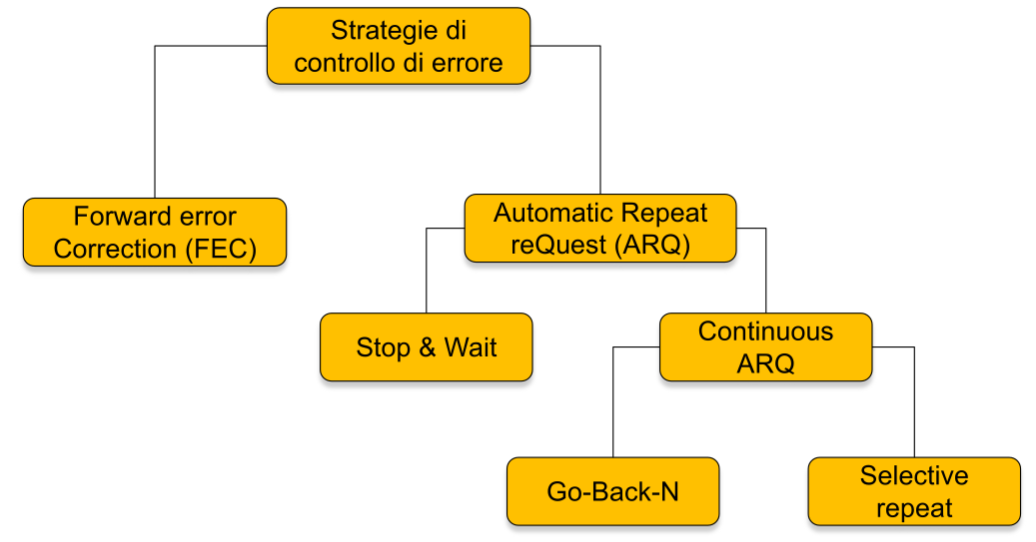
\includegraphics[width=0.7\textwidth]{images/strategierrore.png}
    \caption{Strategie di controllo degli errori: confronto tra FEC e ARQ}
\end{figure}

\subsection{Protocolli ARQ (Automatic Repeat-reQuest)}
Nei sistemi di telecomunicazioni, Automatic Repeat-reQuest è una strategia di controllo di errore, che svolge il compito di rivelare un errore (ma non di correggerlo). I pacchetti corrotti vengono scartati e viene richiesta la loro ritrasmissione.
I protocolli di tipo ARQ più comuni sono:

\begin{multicols}{3}
\begin{itemize}
    \item Stop-and-Wait 
    \item Go-Back-N 
    \item Selective Repeat
\end{itemize}
\end{multicols}


\newpage
\subsubsection{Stop-and-Wait}
Lo stop-and wait è un protocollo di tipologia Continous ARQ, per cui è ammessa la trasmissione continua di più frame numerati.

In questo caso specifico, i segnali di riscontro negativi sono cumulativi.

\begin{figure}[htbp]
    \centering
    \begin{minipage}{0.4\textwidth}
        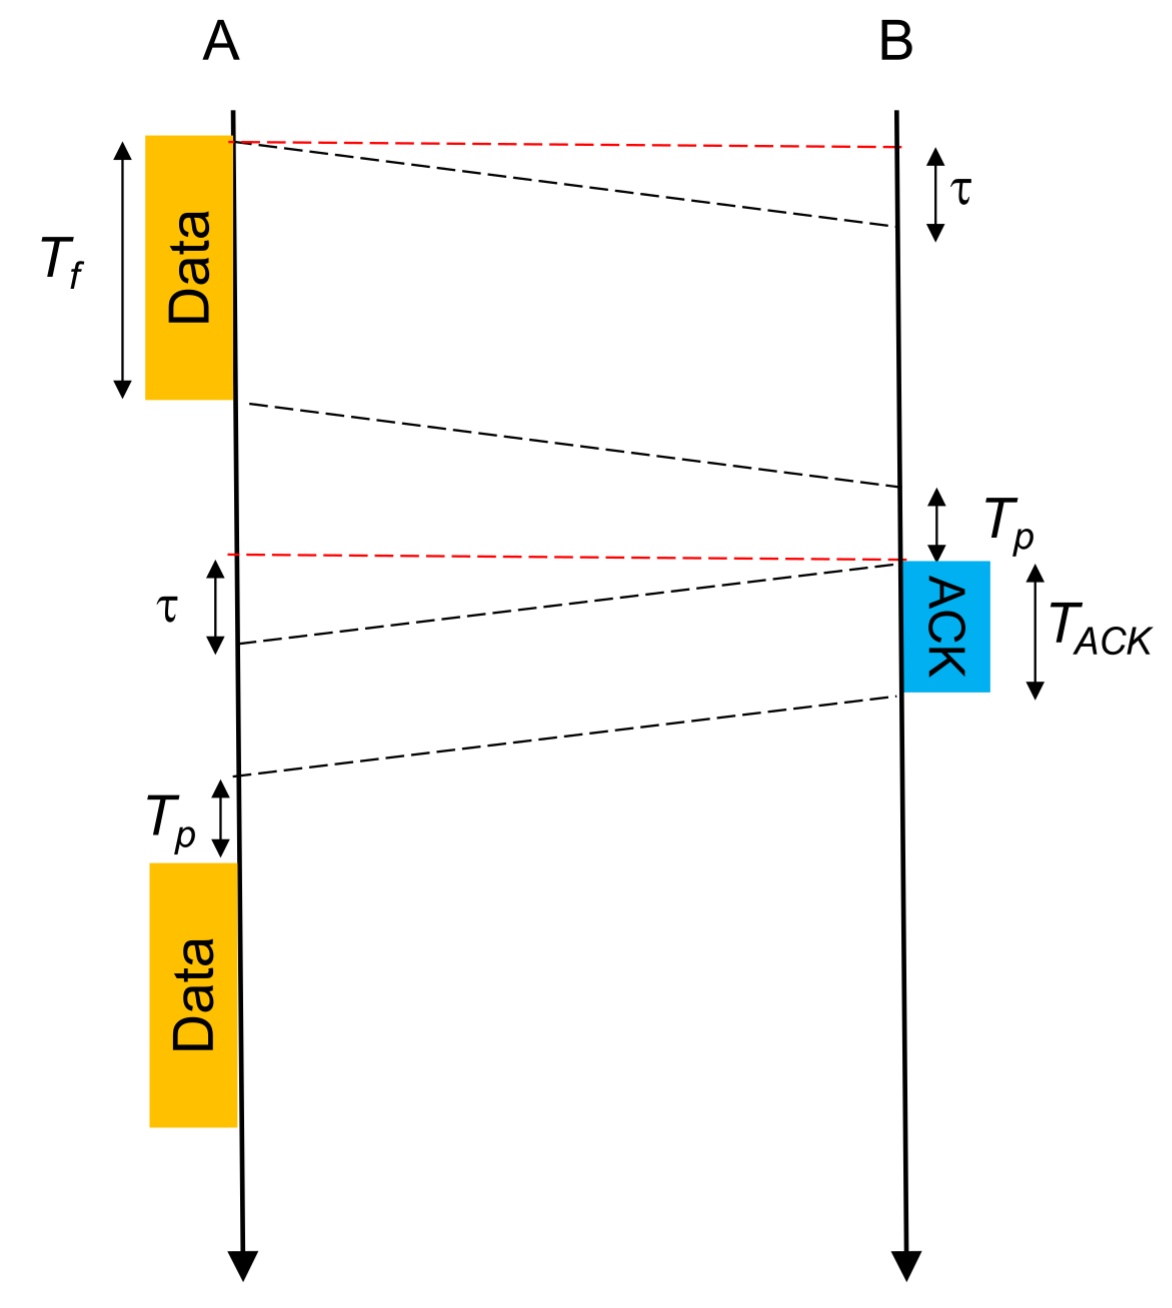
\includegraphics[width=\linewidth]{images/stopwait.png}
        \caption{Schema Stop-and-Wait}
    \end{minipage}%
    \hfill
    \begin{minipage}{0.55\textwidth}
        Il protocollo Stop-and-Wait prevede che il mittente attenda il riscontro del destinatario per ogni frame inviato, prima di procedere con il frame successivo.

        Il mittente invia una trama, quindi si ferma (stop) e attende (wait) il riscontro (Ack) da parte del ricevente prima di trasmettere una nuova trama.
\begin{itemize}
    \item $T_f$: tempo di trasmissione di una trama [s]
    \item $T_{ACK}$: tempo di trasmissione di un riscontro [s]
    \item $T_p$: tempo di elaborazione di una trama [s]
    \item $\tau$: tempo di propagazione [s]
\end{itemize}
    \end{minipage}
\end{figure}

\paragraph{Efficienza di stop and wait in assenza di errori}

Prima di definire l'efficienza del protocollo, è necessario definire il tempo necessario a trasmettere una trama:

\begin{equation}
T_{tot} = T_f + T_{ACK} + 2T_p + 2\tau
\end{equation}

$T_p$ come già detto è il tempo di elaborazione della trama, dipende dalla valocità di elaborazione e quindi non dovrebbe essere precisamente uguale in trasmissione e ricezione, ma per semplicità lo consideriamo uguale.
Inoltre $T_f$, il tempo di trasmissione della trama, è anche definito come il tempo utile, poichè tutti gli altri tempi che consideriamo sono relativi a operazioni di controllo,elaborazione e invio del pacchetto
L'efficienza ($\eta$) è perciò definita come:
\begin{equation}
\eta = \frac{T_f}{T_{tot}} = \frac{T_f}{T_f + T_{ACK} + 2T_p + 2\tau}
\end{equation}

Si possono effettuare alcune semplificazioni, considerando che $T_{ACK}$ e $T_p$ sono molto più piccoli di $T_f$ e $\tau$, quindi possiamo considerare:

\begin{equation}
T_{tot} = T_f + 2\tau
\end{equation}
da cui si ottiene l'efficienza:

\begin{equation}
\eta = \frac{T_f}{T_f + 2\tau} = \frac{1}{1 + \frac{2\tau}{T_f}} = \frac{1}{1 + \alpha} 
\end{equation}
dove $\alpha$ = $\frac{2\tau}{T_f}$ è il rapporto di propagazione normalizzato

\begin{itemize}
    \item il throughput è pari al prodotto tra la frequenza di cifra C (capacità del canale) e l'efficienza: $\eta$C
    \item anche in assenza di errori, l'efficienza non è mai pari a 1.
\end{itemize}

\newpage

\paragraph{Efficienza di stop and wait in presenza di errori}

I problemi che possono verificarsi sono:
\begin{multicols}{2}
\begin{itemize}
    \item il frame o l'ACK arrivano errati
    \item il frame non arriva
\end{itemize}
\end{multicols}

\begin{figure}[htbp]
    \centering
    \begin{minipage}{0.48\textwidth}
        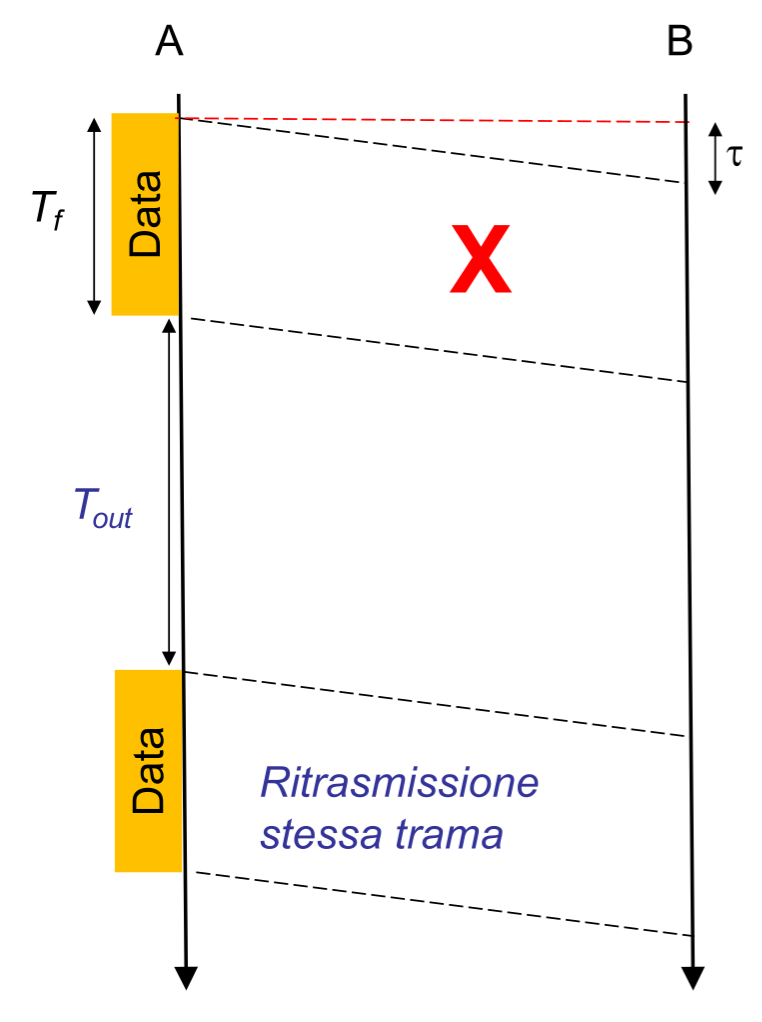
\includegraphics[width=\linewidth]{images/erroreframe.png}
        \caption{Errore nel frame: quando si verifica un errore nel frame, il mittente si accorge del problema grazie alla scadenza del timer avviato durante la trasmissione. 
        In tal caso, il frame viene ritrasmesso. Questo processo garantisce che i dati vengano ricevuti correttamente, ma può ridurre l'efficienza del protocollo a causa delle ritrasmissioni necessarie.}
    \end{minipage}%
    \hfill
    \begin{minipage}{0.48\textwidth}
        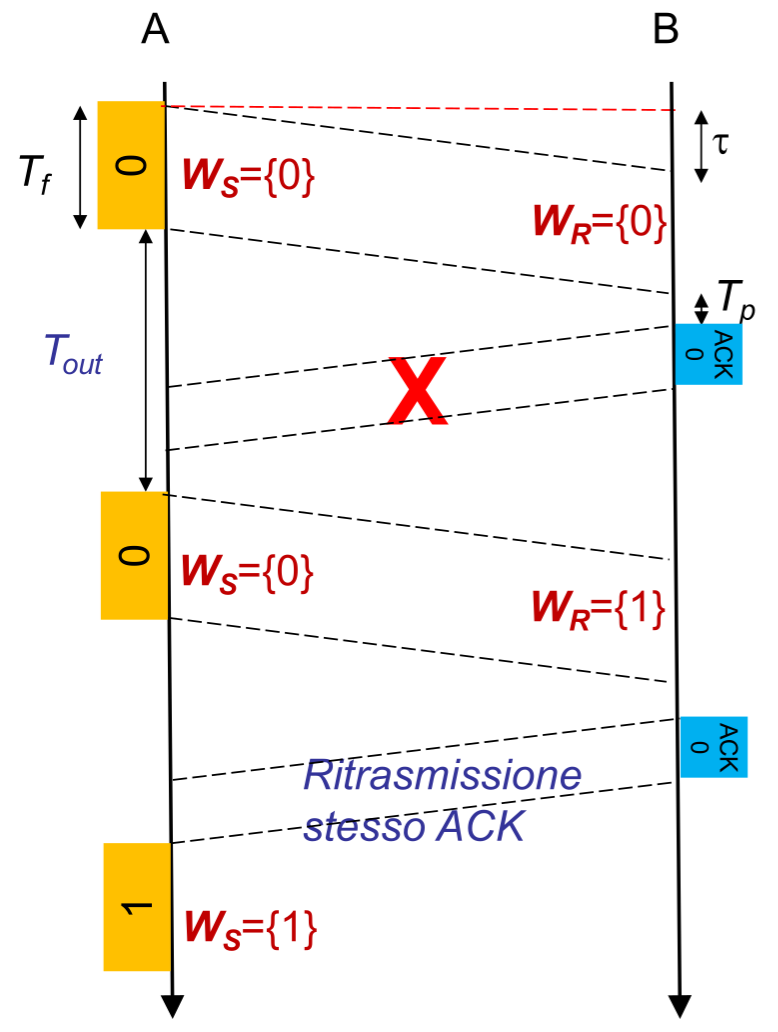
\includegraphics[width=\linewidth]{images/erroreack.png}
        \caption{Errore nell'ACK: quando si verifica un errore nell'ACK, il mittente non riceve il riscontro atteso entro il tempo stabilito dal timer. 
        Anche in questo caso, il frame viene ritrasmesso. }
    \end{minipage}
\end{figure}

Come calcolo il $T_{out}$(time che avvio nel momente nella trasmissione del frame)?

Deve valere almeno il tempo di invio del ACK($T_{ACK}$), più il tempo di propagazione(andata e ritorno) più il tempo di elaborazione del frame($T_p$, in ricezione e trasmissione):
\begin{equation}
T_{out} \geq T_{ACK} + 2\tau + 2T_p
\end{equation}

Il numero di frame ritrasmessi per la corretta ricezione del frame è detto $N_S$ ed è in media considerabile come una variabile aleatoria;

inoltre il numero totale di frame trasmessi($N_R$) è dato dal numero di frame ritrasmessi più il frame inviato con successo:
\begin{equation}
N_R = N_S + 1
\end{equation}


Definiamo il frame error rate(FER), come la probabilità che un frame venga ricevuto con errore, FINIRE E APPROFONDIRE

\newpage
\subsection{Protocolli Continuous ARQ}
I protocolli continuous ARQ, a differenza dello stop-and-wait, prevede l'invio di un'insieme di pacchetti(frame/trame) numerati, tramite sliding window.
Vengono definite:
\begin{itemize}
    \item finestra di trasmissione $W_s$: definisce la grandezza della finestra di ricezione, perciò quanti pacchetti posso inviare "consecutivamente"(on the fly, in attesa di riscontro) e da cui posso aspettarmi un riscontro (ACK) cumulativo
    \item finestra di ricezione  $W_R$: definisce la grandezza della finestra di ricezione, 
\end{itemize} 
Se il campo dedicato alla numerazione è costituito da b bit, si potranno
numerare in modo differente fino a $N_b$ trame. 


\subsubsection{Go-Back-N}
\paragraph{Senza errori - efficienza massima}
Il protocollo Go-Back-N è un protocollo di tipo Continuous ARQ, che consente la trasmissione continua di più frame numerati. In questo caso specifico, i segnali di riscontro negativi sono cumulativi.

Nel caso in cui ci siano errori allora questo protocollo prevede di ritornare indietro nel momento della trasmissione in cui c'è stato l'errore(alla trama N), perciò go back N.
\begin{figure}[htbp]
    \centering
    \begin{minipage}{0.4\textwidth}
        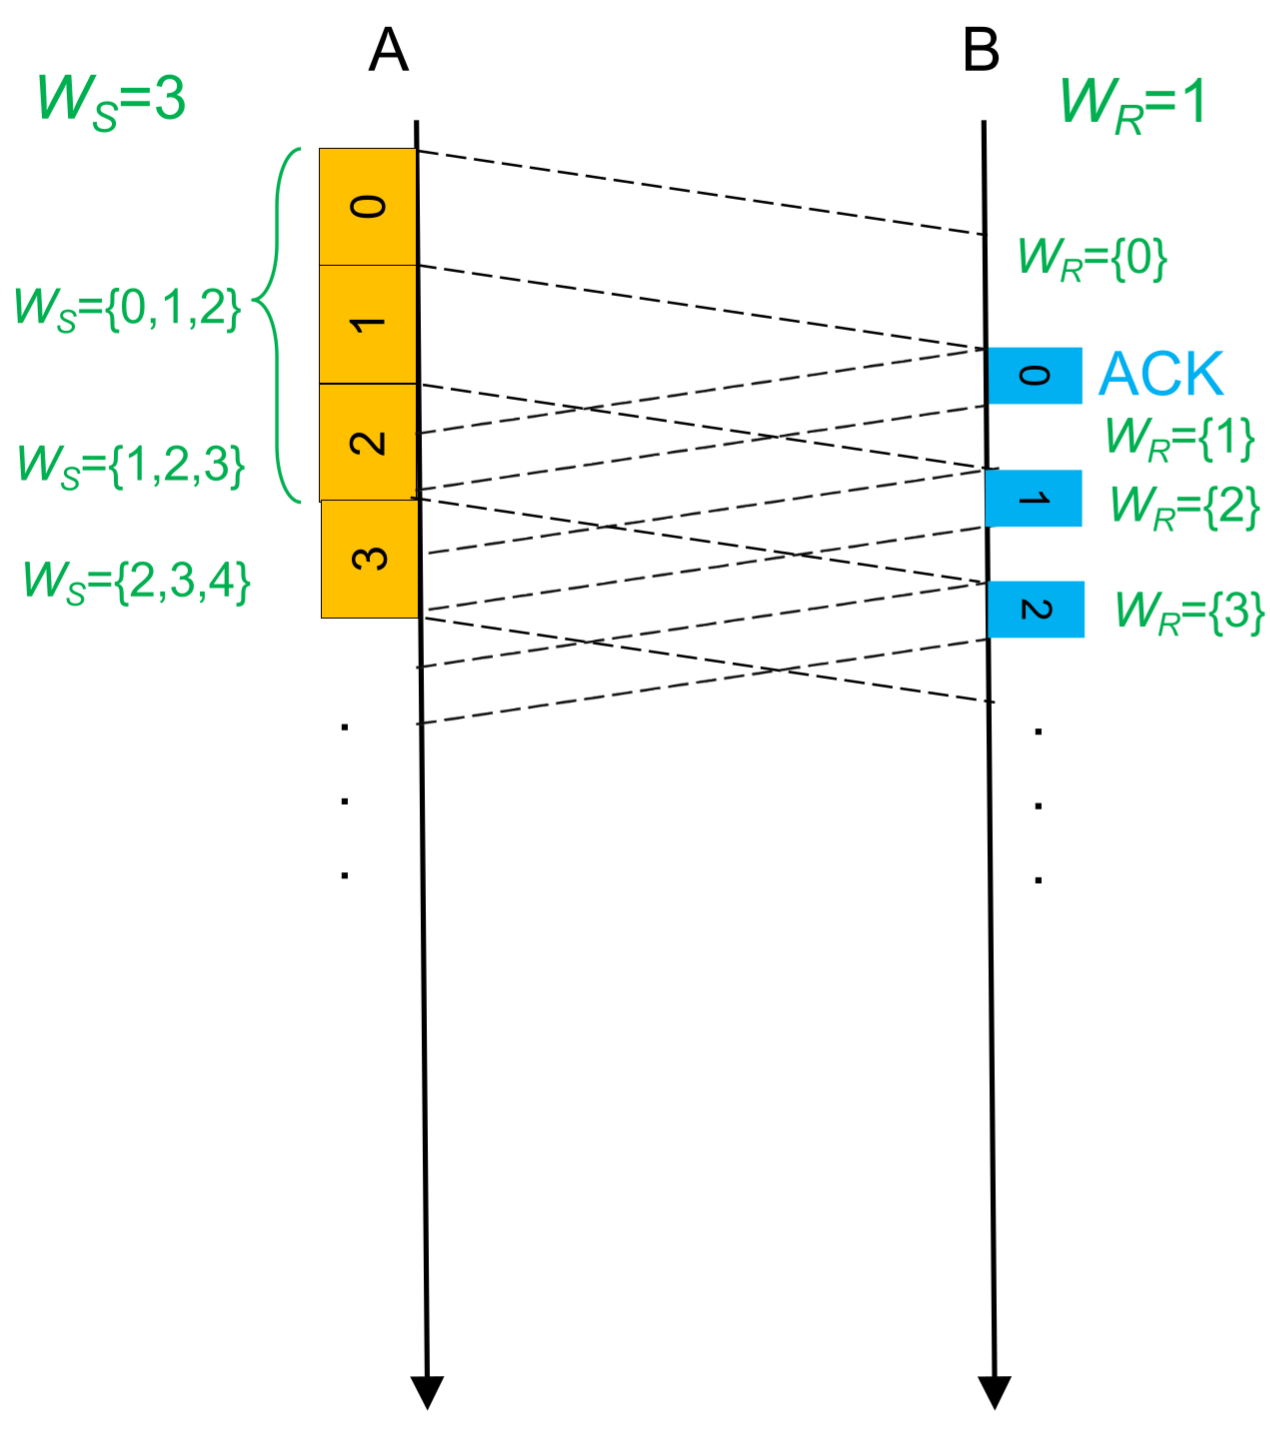
\includegraphics[width=\linewidth]{images/gobackinsenzaerrori.png}
        \caption{Go-Back-N senza errori}
    \end{minipage}%
    \hfill
    \begin{minipage}{0.55\textwidth}
        Nel seguente esempio la finestra di tramissione è 3 e quella di ricezione 1; vengono riscontrati gli ack in modo corretto nei tempi previsti dalla finestra, che nel frattempo ad ogni ack corretto ricevuto scorre di posizione.
        
        Questo vuol dire che nel caso in cui non ci siano errori con l'invio delle trame e con il riscontro degli ack, il seguente protocollo ha efficienza massima.
 
    \end{minipage}
\end{figure}
 \newpage
\subsubsection{Con errori}
Si possono riscontrare errori durante la ricezione del pacchetto e durante il riscontro degli ack; a seconda della tipologia dell'errore avremo soluzioni differenti.
\paragraph{Errore trasmissione del frame} utilizzo del negative ACK (NACK)
\begin{figure}[htbp]
    \centering
    \begin{minipage}{0.4\textwidth}
        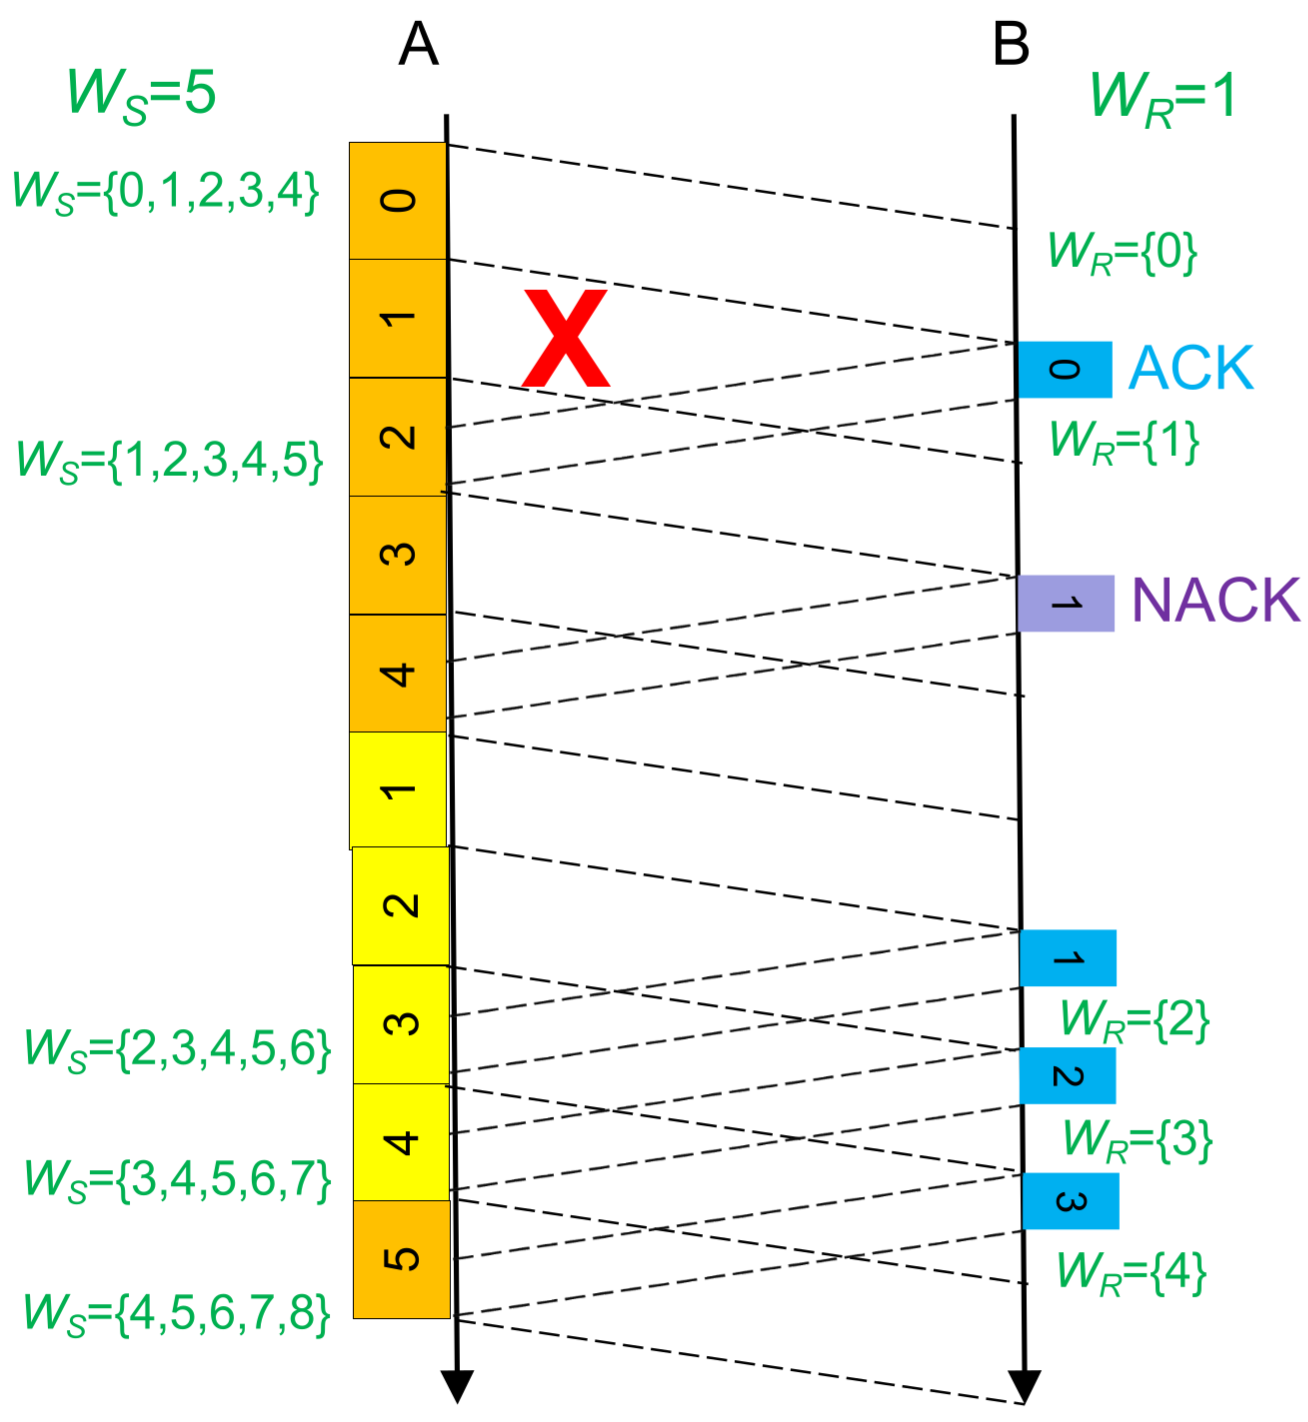
\includegraphics[width=\linewidth]{images/gobackinerrori.png}
        \caption{Go-Back-N con errori in trasmissione}
    \end{minipage}%
    \hfill
    \begin{minipage}{0.55\textwidth}
        Quando si verifica un errore in un frame, il destinatario scarta il frame errato e tutti i frame successivi. 
        
        Il mittente, una volta rilevato l'errore(tramite la ricezione di un NACK(negative ACK) inviato dal destinatario), ritrasmette il frame errato e tutti i frame successivi.
    \end{minipage}
\end{figure}

\paragraph{Errore trasmissione - ACK non ricevuto ($T_{out}$)} caso in cui l'ACK non venga inviato o si sia perso

\begin{figure}[htbp]
    \centering
    \begin{minipage}{0.55\textwidth}
        L'unico modo con il quale il mittente può evitare che il sistema si blocchi in caso di mancato riscontro(neanche NACK),  è quello di avviare un timer ad ogni frame inviato, entro il quale va ricevuto un riscontro.
        
        Se questo timer($T_{out}$) scade allora la finestra torna indietro e ritrasmette da dove è stato riscontrato il problema.
    \end{minipage}%
    \hfill
    \begin{minipage}{0.4\textwidth}
        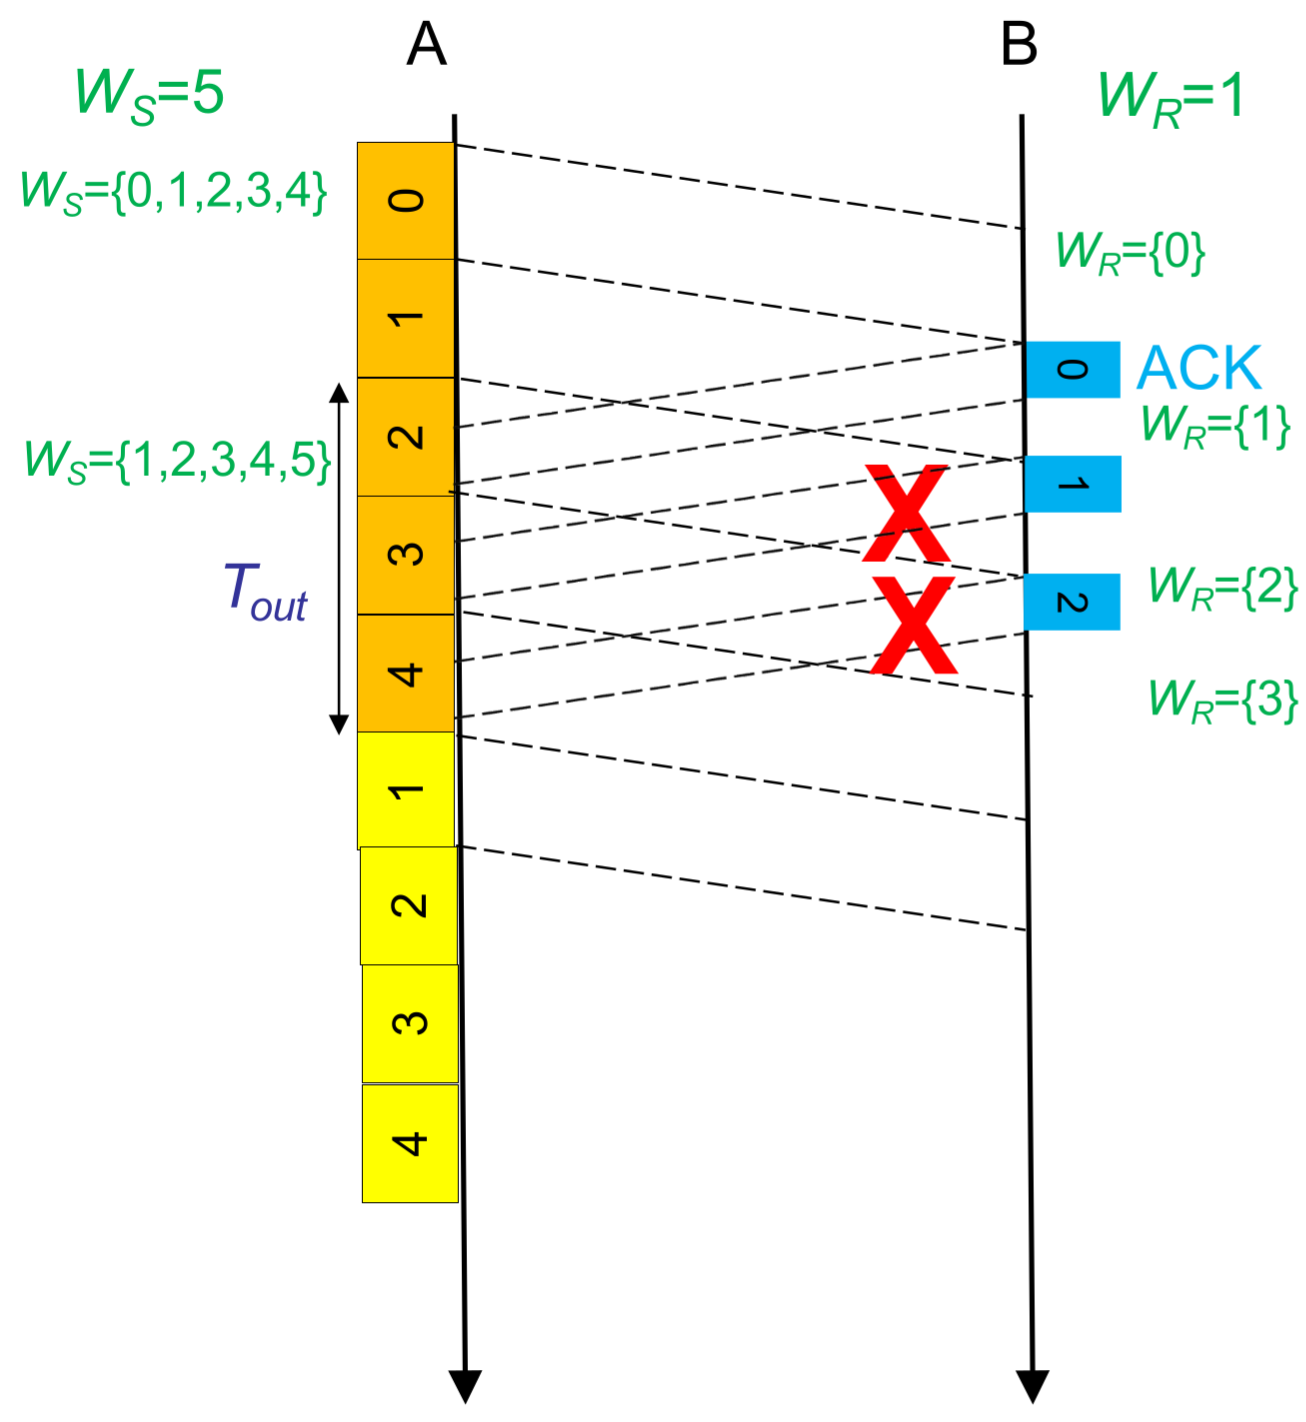
\includegraphics[width=\linewidth]{images/gobacknerroreack.png}
        \caption{Go-Back-N con errore nell'ACK}
    \end{minipage}
\end{figure}

\newpage

\paragraph{Errore trasmissione - ACK equivocato($T_{out}$)} 
con conseguente ricezione di duplicati

\begin{figure}[htbp]
    \centering
    \begin{minipage}{0.5\textwidth}
        Quando si verifica un equivoco nell'ACK,ossia viene riscontrato erroneamente un frame,  il mittente interpreta erroneamente il riscontro ricevuto e potrebbe ritrasmettere frame già ricevuti correttamente dal destinatario. 
        Questo equivoco può portare a un aumento delle ritrasmissioni e a una riduzione dell'efficienza del protocollo.

        Questi equivoci possono portare ad una sovrapposizione tra le finestre di trasmissione e ricezione; 
    \end{minipage}%
    \hfill
    \begin{minipage}{0.45\textwidth}
        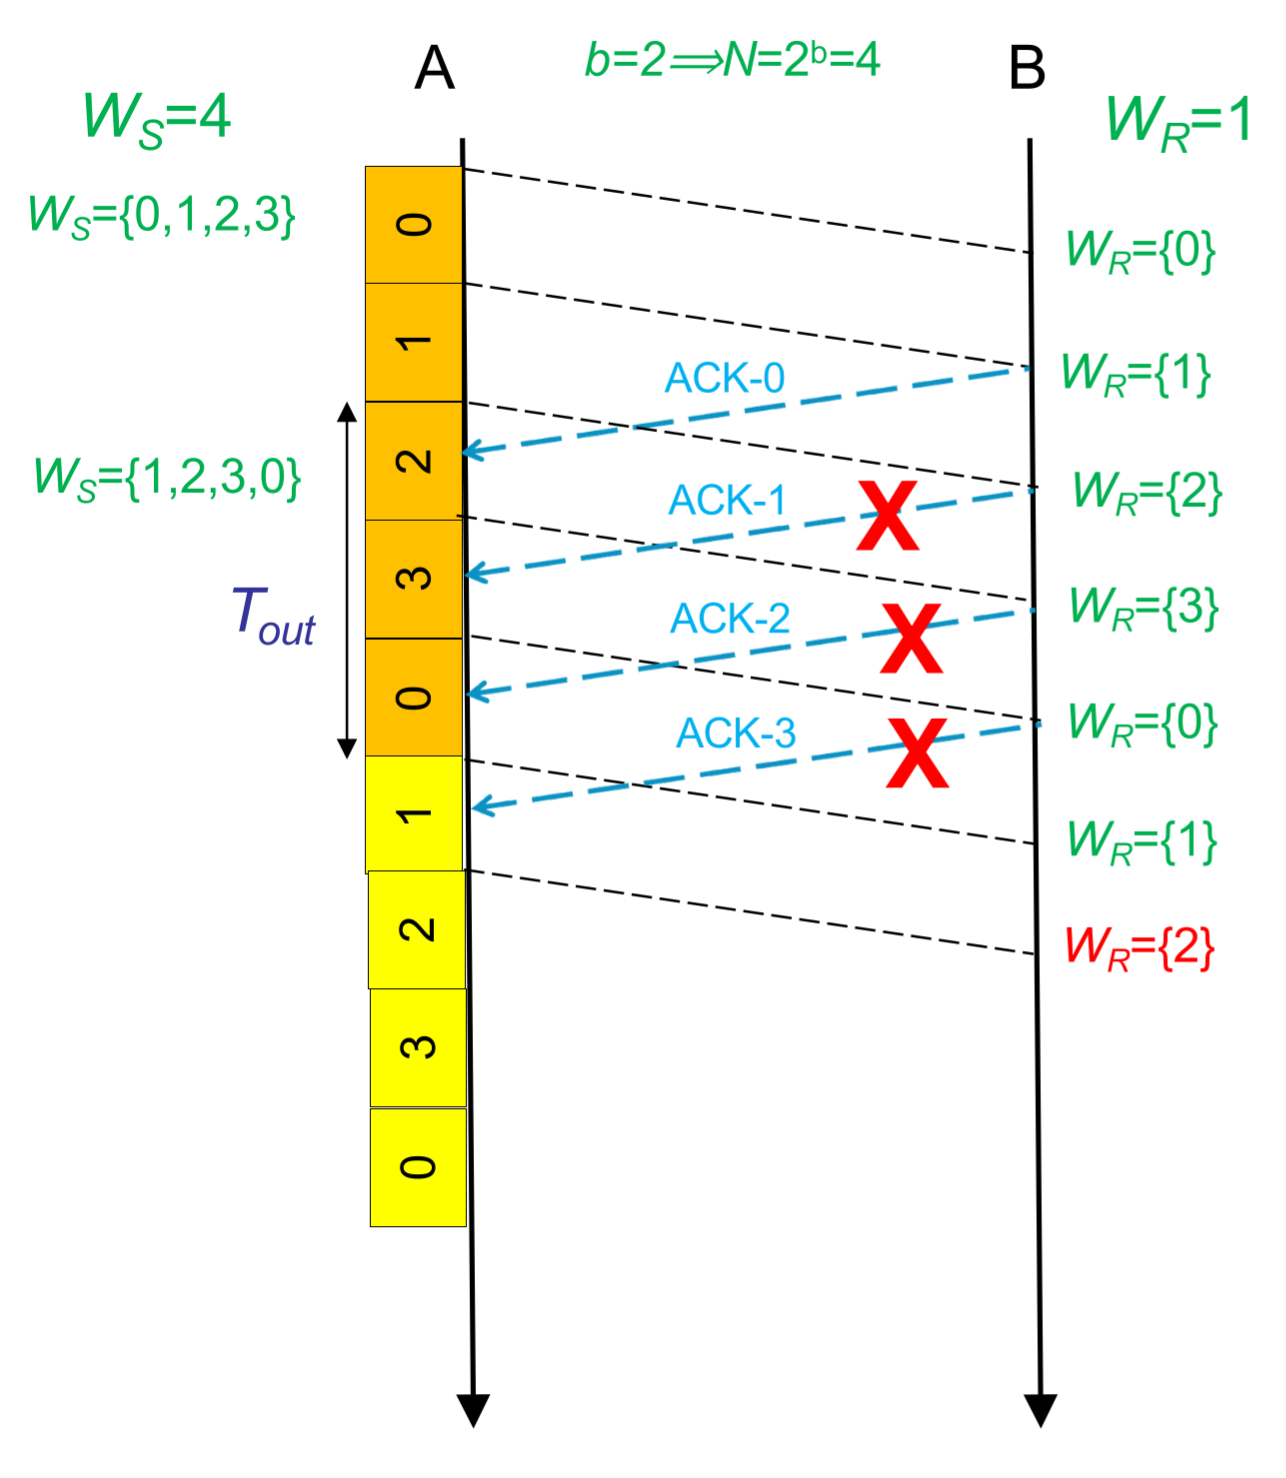
\includegraphics[width=\linewidth]{images/equivocoack.png}
        \caption{Go-Back-N con equivoco nell'ACK}
    \end{minipage}
\end{figure}


\begin{figure}[htbp]
    \centering
     \begin{minipage}{0.46\textwidth}
        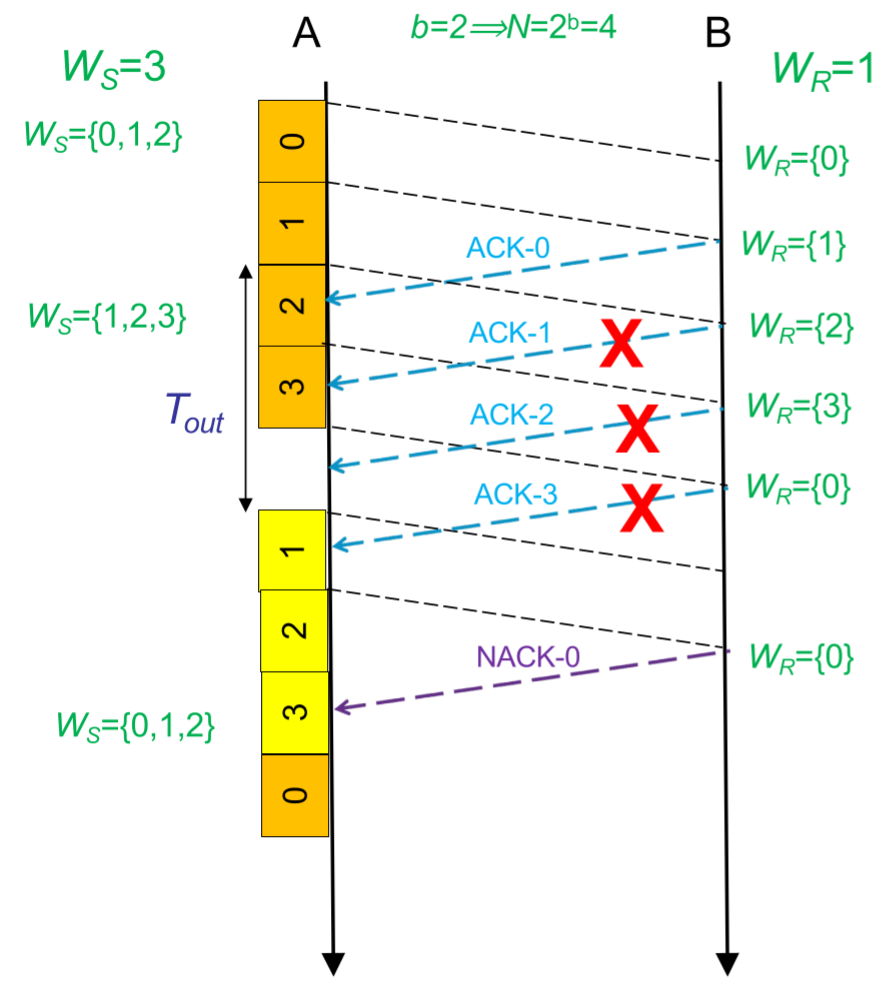
\includegraphics[width=\linewidth]{images/ackequivoco2.png}
        \caption{Go-Back-N con equivoco nell'ACK}

    \end{minipage}
    \hfill
    \begin{minipage}{0.5\textwidth}
        DA FARE
    \end{minipage}%
\end{figure}
\newpage

\paragraph{Protocollo selective repeat} 
Il protocollo Selective Repeat è un protocollo di tipo Continuous ARQ che consente la ritrasmissione selettiva dei soli frame ricevuti con errore, evitando di ritrasmettere quelli ricevuti correttamente.


        \begin{figure}[htbp]
    \centering
    \begin{minipage}{0.47\textwidth}
        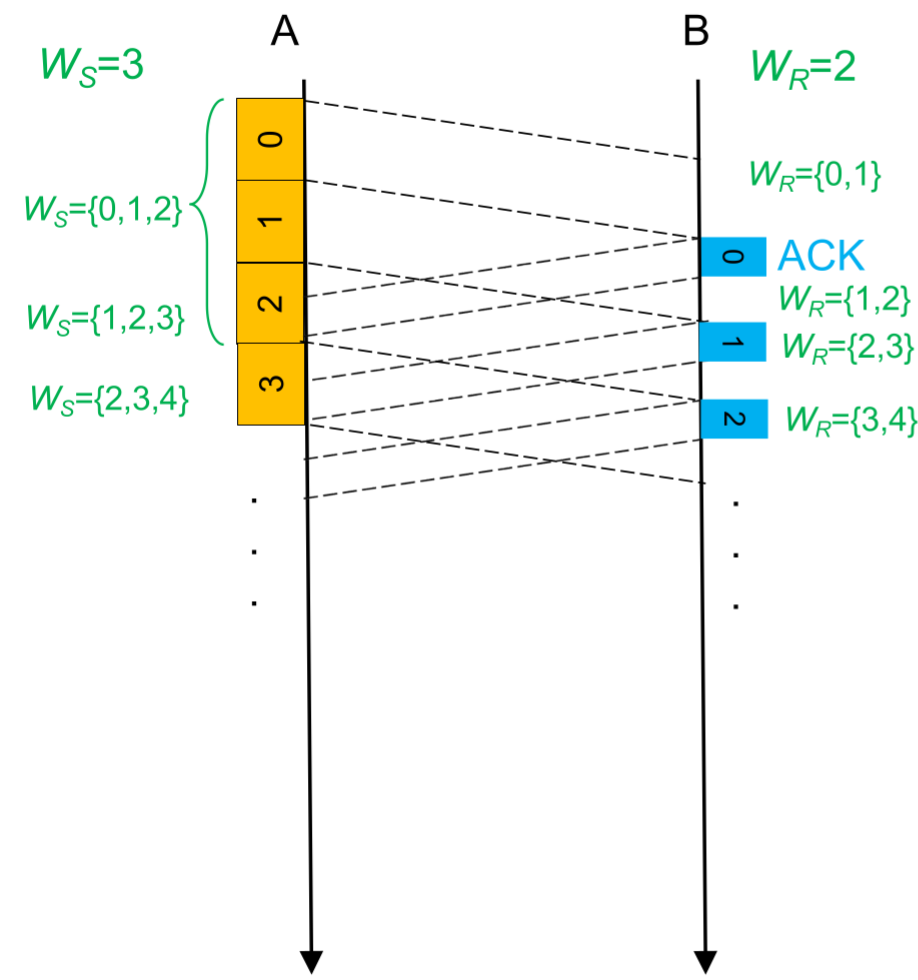
\includegraphics[width=\linewidth]{images/sr.png}
        \caption{Selective Repeat}
        
    \end{minipage}%
    \hfill
    \begin{minipage}{0.48\textwidth}
        \paragraph{In assenza di errori} Questo approccio migliora l'efficienza rispetto al Go-Back-N, poiché la finestra di ricezione può essere maggiore di 1 ($W_R > 1$).

    \end{minipage}
\end{figure}


\begin{figure}[htbp]
    \centering
    \begin{minipage}{0.47\textwidth}
        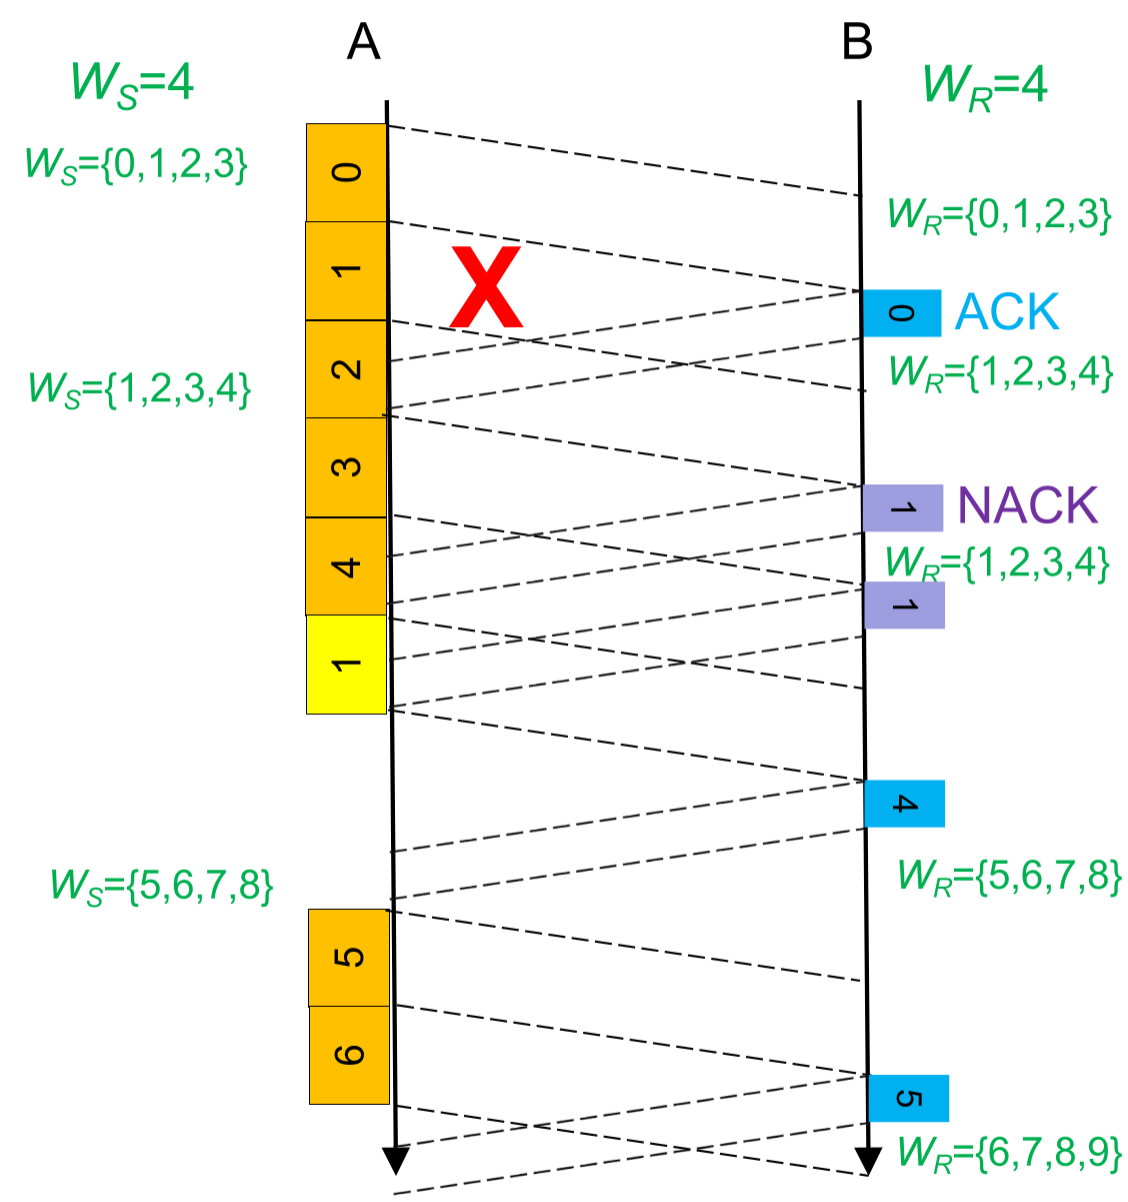
\includegraphics[width=\linewidth]{images/srerroritrama.png}
        \caption{Selective Repeat con errori sulla trama}
    \end{minipage}%
    \hfill
    \begin{minipage}{0.49\textwidth}
        \paragraph{In presenza di errori sulla trama}

        Quando si verifica un errore in una trama, il protocollo Selective Repeat consente di ritrasmettere solo la trama errata(il ricevente invia un NACK in cui indica quale frame è andato perso), senza dover ritrasmettere tutte le trame successive come avviene nel Go-Back-N. 
        

        Questo approccio riduce il numero di ritrasmissioni necessarie e migliora l'efficienza complessiva del protocollo, specialmente in presenza di errori frequenti.
    \end{minipage}
\end{figure}
\newpage
\begin{figure}[htbp]
    \centering
    \begin{minipage}{0.5\textwidth}
        \paragraph{In presenza di errori sull'ACK}
        Quando si verifica un errore nell'ACK, il protocollo Selective Repeat consente di gestire la situazione senza dover ritrasmettere tutte le trame successive. 
        Il mittente ritrasmette solo le trame per cui non ha ricevuto un riscontro positivo, evitando duplicati e migliorando l'efficienza rispetto al Go-Back-N.
    \end{minipage}%
    \hfill
    \begin{minipage}{0.47\textwidth}
        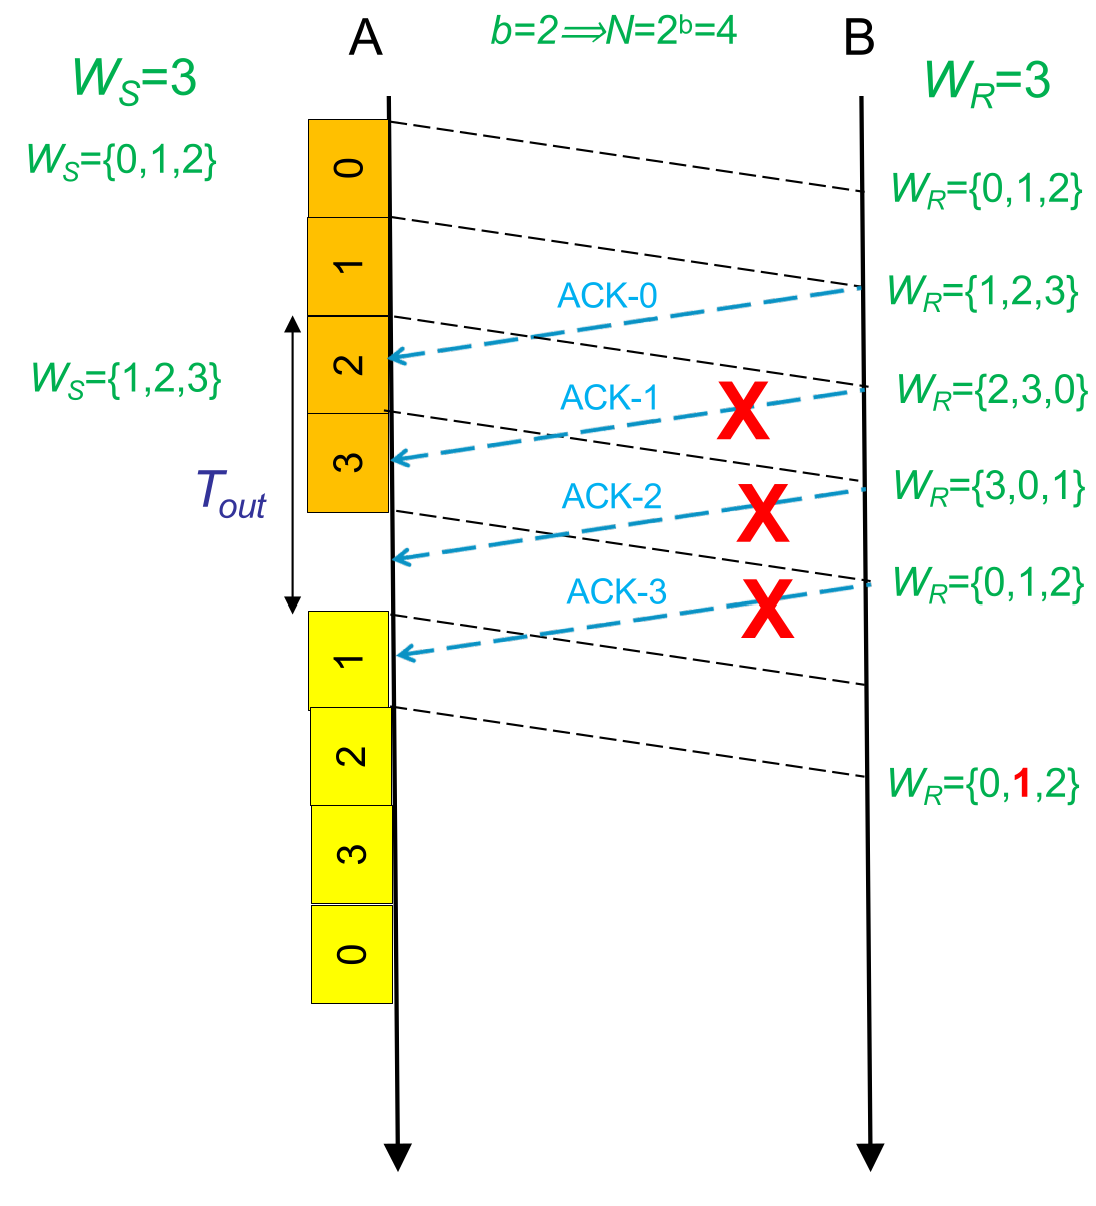
\includegraphics[width=\linewidth]{images/srequivocazione.png}
        \caption{Selective Repeat con errori sull'ACK}
    \end{minipage}
\end{figure}